\documentclass[slidetop,11pt]{beamer}
\graphicspath{{Images/}}
\usepackage[T1]{fontenc}
\usepackage{graphicx}
\usepackage{multimedia}
\usepackage[utf8]{inputenc}
\usepackage[frenchb]{babel}
\usepackage{url,qrcode}
\usepackage{hyperref}


\def\R{\mathbb{R}}
\def\Z{\mathbb{Z}}
\def\bS{\mathbb{S}}
\def\cC{\mathcal{C}}
\def\HH{\mathbb{H}}
\def\cH{\mathcal{H}}
\def\bd{\partial}


\usetheme{JuanLesPins}
\usecolortheme{seahorse}

\title{Magistère de Mathématiques Poincaré\\ Présentation de la formation}
\author{D. Mégy}
%\institute{Institut élie Cartan de Lorraine, UMR 7752}
%\logo{
\includegraphics[height=1cm]{Logo-MMP-noir-2}}


\begin{document}


  
%\begin{frame}
%\titlepage
%\end{frame}

\begin{frame}
\begin{center}

\includegraphics[height=7cm]{images/Logo-MMP-noir-cropped}
\end{center}
\end{frame}  

\begin{frame}
\frametitle{Table des matières}
\tableofcontents
\end{frame}

\section{Présentation générale de la formation}

\begin{frame}
\begin{center}

\includegraphics[height=1.5cm]{images/Logo-MMP-noir-2}
\end{center}
Le \textbf{Magistère de Mathématiques Poincaré} est une formation sélective de haut niveau de \textbf{3 ans} proposée à \textbf{Nancy} et accessible sur dossier après une deuxième année de licence de mathématiques (L2) ou deux années de classes préparatoires, englobant le cursus L3, M1, M2 classique.
\bigskip

En plus des diplômes nationaux de la \textbf{Licence} et du \textbf{Master}, la formation est sanctionnée par un \textbf{diplôme universitaire de Magistère}, délivré lors de l'obtention du Master.
\end{frame}

\begin{frame}
Le Magistère de Mathématiques Poincaré s'appuie sur l'environnement scientifique de la recherche faite à l'Institut Elie Cartan de Lorraine (IECL) et propose une palette d'activités enrichissant le cursus classique licence/master prévoyant entre autres :
\begin{itemize}
\item 5 enseignements supplémentaires sous la forme de cours classiques.
\item Un mémoire d'initiation à la recherche au niveau L3.
\item Un stage d'application des mathématiques en M1.
\item Deux « Masterclasses » une en M1, une en M2.
\item Un séminaire du Magistère mensuel d'initiation à la recherche.
\item Des séances de problèmes d'écrits de concours.
\end{itemize}

\end{frame}


 
 \section{Première année de Magistère}
\begin{frame}
\frametitle{Magistère 1A : cours communs de Licence S5}
\begin{itemize}
\item \textbf{Algèbre 3} (6 ECTS) : théorie des groupes jusqu'aux théorèmes de Sylow
\item \textbf{Intégration et probabilités} (9 ECTS) : théorie de la mesure, intégrale de Lebesgue, variables aléatoires mesurables
\item \textbf{Topologie et analyse hilbertienne} (6 ECTS) : Topologie, espaces fonctionnels, espaces de Hilbert
\item Une option (6 ECTS) parmi \textbf{Calcul formel} (arithmétique, cryptographie, corps finis) et \textbf{Analyse numérique} (analyse numérique matricielle, LU, QR...)
\item \textbf{Anglais}, et \textbf{Mathématiques en anglais} (3 ECTS)
\end{itemize}

\end{frame}

\begin{frame}
\frametitle{Magistère 1A : cours communs de Licence S6}


\begin{itemize}
\item \textbf{Algèbre 4} (6 ECTS) : anneaux, corps, polynômes symétriques, arithmétique
\item \textbf{Analyse complexe} (6 ECTS) : fonctions holomorphes, théorie de Cauchy, résidus, Rouché
\item \textbf{Calcul différentiel} (6 ECTS) : calcul différentiel dans un Banach : inversion locale, EDO, Cauchy-Lipschitz
\item \textbf{Probabilités et statistique} (9 ECTS) : convergence des v.a., transformée de Fourier, théorème central limite, estimateurs.
\item \textbf{TIPE/Stage} (3 ECTS) : stage d'initiation à la recherche en mathématiques en laboratoire, mémoire et soutenance
\item \textbf{Anglais} et \textbf{Mathématiques en anglais} (3 ECTS)
\end{itemize}
\end{frame}

\begin{frame}
\frametitle{Magistère 1A : cours supplémentaires de Magistère (S5)}

\textbf{Analyse harmonique et applications en théorie des nombres} (6 ECTS, 30hCM+30hTD)

Ce cours comportera deux parties, l'une de présentation de l'analyse de Fourier et l'autre d'application à la théorie analytique des nombres, dont une preuve du célèbre théorème des nombres premiers.
\begin{center}
\includegraphics[scale=.2]{images/fourier2.jpg} 
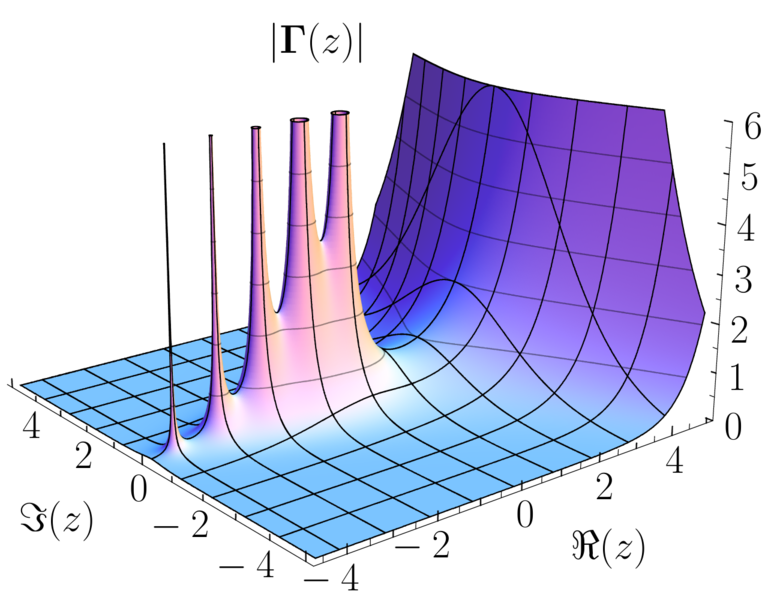
\includegraphics[scale=.2]{images/Gamma_abs_3D.png}
% image wikipedia https://en.m.wikipedia.org/wiki/File:Gamma_abs_3D.png
% trouver une image mieux adaptée, plus analyse harmonique qu'analyse complexe
\end{center}

\end{frame}

\begin{frame}
\frametitle{Magistère 1A : cours supplémentaires (S6)}

\textbf{Mécanique quantique} (3 ECTS, 14h CM+16h TD)

L'objectif de ce cours est d'introduire la théorie de la mécanique quantique (relation d'incertitudes, processus de mesures) et ses implications.
\begin{center}
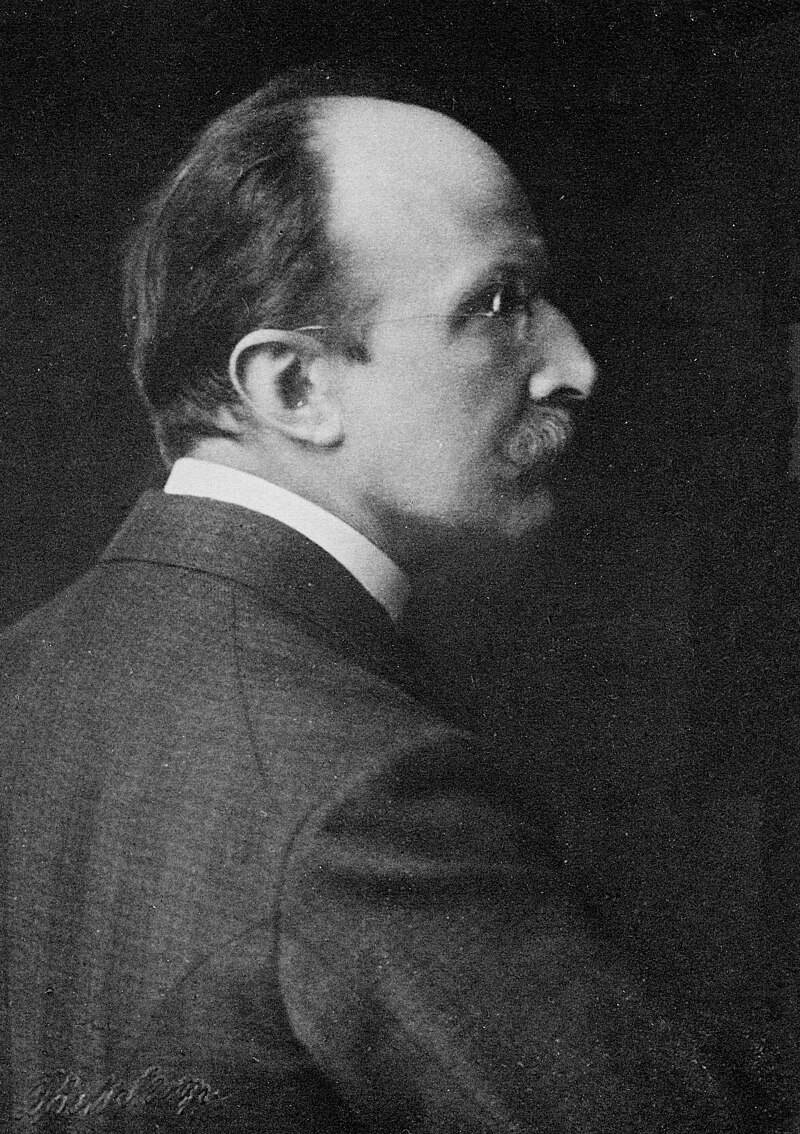
\includegraphics[height=4.3cm]{Max_Planck_Nobel_1918.jpg}$\quad$
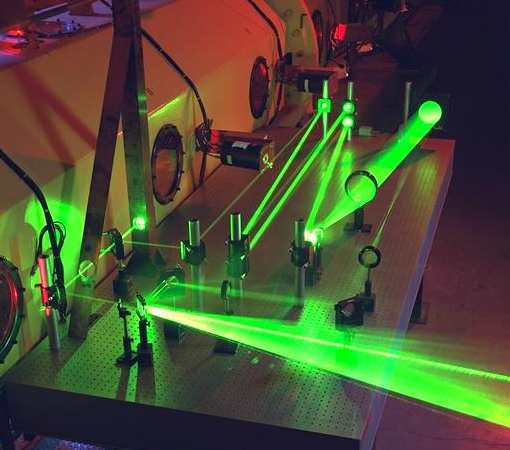
\includegraphics[height=4.3cm]{Laser_optique.jpg}
% source : wikipedia page mecanique quantiqe et max Planck
\end{center}
\end{frame}

\begin{frame}
\frametitle{Magistère 1A : cours supplémentaires (S6)}

\textbf{Équations différentielles : géométrie, dynamique et chaos}\\
(3 ECTS, 16hCM+14h TD)

Dans ce cours, nous explorerons les bases des systèmes dynamiques, aussi appelées \og théorie du chaos\fg, avec pour fil conducteur un célèbre article du physicien Lorenz qui introduisit la notion d'effet papillon.
\begin{columns}[c]
\begin{column}{6cm}
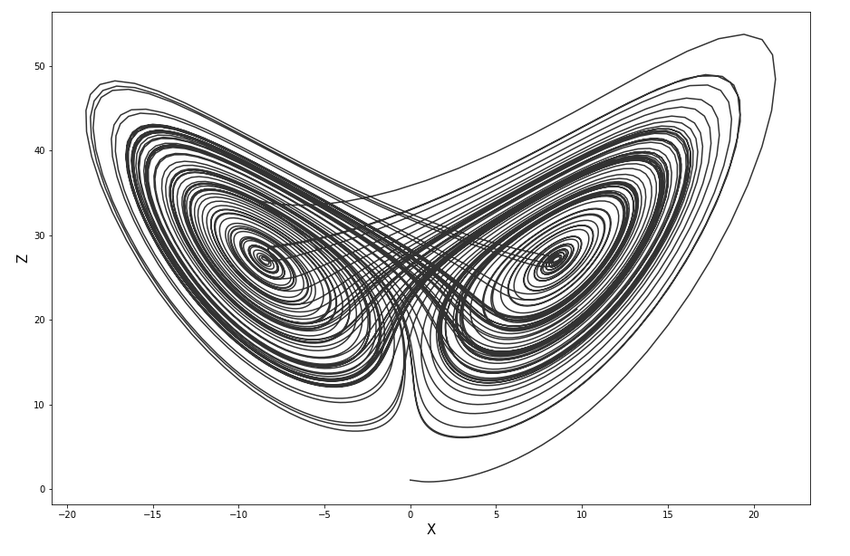
\includegraphics[scale=.2]{images/Lorenz-Attractor-in-2D-space.png}
% crédits : Anton Koshelev DOI:10.48550/arXiv.2104.14190
% image en CCBY NC, rajouter la référence
% trouver une meilleure image...
\end{column}
\begin{column}{5cm}
Vidéo d'introduction: \\
\url{www.chaos-math.org}\\
\qrcode{https://www.chaos-math.org/fr.html}
\end{column}
\end{columns}


\end{frame}

\begin{frame}
\frametitle{Magistère 1A : activités supplémentaires de Magistère}
\end{frame}

 \section{Deuxième année de Magistère}
\begin{frame}
\frametitle{Deuxième année de Magistère}

\end{frame}


 \section{Troisième année de Magistère}
\begin{frame}
\frametitle{Troisième année de Magistère}

\end{frame}


\begin{frame}
\frametitle{Questions ?}

\begin{center}
{\LARGE \bf Merci pour votre attention !!}

\bigskip
\qrcode[hyperlink, height=4cm]{https://iecl.univ-lorraine.fr/magistere-poincare}

\bigskip
\url{https://iecl.univ-lorraine.fr/magistere-poincare}
\end{center}
\end{frame}
  \end{document}
  